% !TeX program = lualatex
% !BIB program = biber
% Lualatex is important to render TTF fonts; with pdflatex it's just the regular one
% ratio 16:9 -- https://tex.stackexchange.com/questions/14336/

% compile two versions, inspired by https://tex.stackexchange.com/a/1501
% use the script "compile-pdf.sh"
\newif\ifhandout
% if flags.tex does not exist, create an empty file to be able to compile in TeXstudio
\input{flags}

\ifhandout
\documentclass[12pt,aspectratio=169,handout]{beamer}
\else
\documentclass[12pt,aspectratio=169]{beamer}
\fi



% TODO change "leftfootertext" to your liking
\newcommand{\leftfootertext}{\insertsubtitle}  % just the \title{} text by default
%\newcommand{\leftfootertext}{AI is all you need | Dr.\ Maria Mustermann}  % Your name, for instance


% ------- RUB specifics ----------
% adjust for 16:9
% https://tex.stackexchange.com/questions/354022/modifying-the-margins-of-all-slides-in-beamer
\setbeamersize{text margin left=0.3cm,text margin right=4.5cm} 


% use Metropolis as the basis theme
\usetheme[subsectionpage=progressbar]{metropolis}
% blocks with background globally
\metroset{block=fill}


\usepackage{fontspec}
% RUB fonts need to be installed
% 'UprightFont = * Light' makes sure that the base font is RubFlama Light, which looks
% lighter than RubFlama Regular (would be too thick for slides)
\setsansfont[Scale=MatchLowercase, UprightFont = * Light, BoldFont = * Bold]{RubFlama}
%\setsansfont{Arial} % Open source alternative if you don't have RubFlama

% RUB color scheme
% Dark blue: 0; 53; 96; #003560
\definecolor{RUBDarkBlue}{RGB}{0, 53, 96}

% Light yellow (table fill, etc.); 238; 250; 196; #EEFAC4
\definecolor{RUBLightYellow}{RGB}{238, 250, 196}

%Light green: 141; 174; 16
\definecolor{RUBLightGreen}{RGB}{141, 174, 16}


\setbeamercolor{titlelike}{fg=RUBDarkBlue}
\setbeamercolor{subtitle}{fg=RUBLightGreen}
\setbeamercolor{separation line}{fg=RUBLightGreen}
\setbeamercolor{frametitle}{bg=white, fg=RUBDarkBlue}

% horizontal line on title page and sections
\setbeamercolor{alerted text}{fg=RUBLightGreen}


% Adjust footer bottom (too large by default)
\setbeamertemplate{footline}{%
  \begin{beamercolorbox}[wd=\textwidth, sep=2ex]{footline}%
    \usebeamerfont{page number in head/foot}%
    \usebeamertemplate*{frame footer}
    \hfill%
    \usebeamertemplate*{frame numbering}
  \end{beamercolorbox}%
}


% Lab name, numbering, etc. in footer
\setbeamertemplate{frame numbering}{TrustHLT --- Prof.\ Dr.\ Ivan Habernal \hspace*{1ex} 
\includegraphics[width=7em]{img/rub-logo.pdf}\hspace*{1ex}}

\setbeamertemplate{frame footer}{\hspace*{1ex}\insertframenumber \hspace*{2ex} \leftfootertext}

% adjust the background to be completely white
\setbeamercolor{background canvas}{bg=white}

% logos on the title page
\titlegraphic{%
	\begin{picture}(0,0)
		\put(435,0){\makebox(0,0)[rt]{
\includegraphics[width=7em]{img/rub-logo.pdf}}}
		\put(435,-170){\makebox(0,0)[rt]{
\includegraphics[width=4em]{img/logo-trusthlt.pdf}}}
		\put(435,-196){\makebox(0,0)[rt]{
\includegraphics[width=9em]{img/logo-rctrust.pdf}}}
	\end{picture}%
}


% show TOC at every section start
\AtBeginSection{
	\frame{
		\vspace{2em}
		\sectionpage
		\hspace*{2.2em}\begin{minipage}{10cm}
			\tableofcontents[currentsection]
		\end{minipage}
	}
}

% TOC without subsection
\setcounter{tocdepth}{1} % only-- part,chapters,sections 

% bullet points: rectangles
\useinnertheme{rectangles}
\setbeamercolor{itemize item}{fg=RUBLightGreen}
\setbeamercolor{itemize subitem}{fg=RUBLightGreen}
% enumerate: blue background for better readability
\setbeamercolor{item projected}{bg=RUBDarkBlue}

% make boxes (example, block, etc.) background lighter for readability
\setbeamercolor{block title}{%
	use=normal text,
	fg=normal text.fg,
	bg=normal text.bg!90!fg % lighter background in block title
}
\setbeamercolor{block body}{
	use={block title, normal text},
	bg=block title.bg!30!normal text.bg % lighter background in block body
}


% RUB colors in blocks
\setbeamercolor{block title alerted}{%
	use={block title, alerted text},
	bg=RUBDarkBlue,
	%fg=RUBLightYellow % looks bad
	fg=white % better contrast
}

\setbeamercolor{block title example}{%
	use={block title, example text},
	fg=RUBLightGreen
}


% ------- end of RUB specifics ----------

% all itemize with pause by default
%\beamerdefaultoverlayspecification{<+->}


% typeset mathematics on serif
\usefonttheme[onlymath]{serif}

% better bibliography using biber as backend
\usepackage[natbib=true,backend=biber,style=authoryear-icomp,maxbibnames=30,maxcitenames=9,uniquelist=false,giveninits=true,doi=false,url=false,dashed=false,isbn=false]{biblatex}
% shared bibliography
\addbibresource{../nlpwdl-bibliography.bib}
% disable "ibid" for repeated citations
\boolfalse{citetracker}



\usepackage{xspace}


% for derivatives, https://tex.stackexchange.com/a/412442
\usepackage{physics}

\usepackage{tikz}
\usetikzlibrary{matrix, positioning}
\usetikzlibrary{angles,quotes} % for angles
\usetikzlibrary{backgrounds} % background
\usetikzlibrary{decorations.pathreplacing} % curly braces
\usetikzlibrary{calligraphy}
\usetikzlibrary{calc} % for neural nets

% for plotting functions
\usepackage{pgfplots}
\usepgfplotslibrary{dateplot}

% sub-figures
\usepackage{caption}
\usepackage{subcaption}

% book tabs
\usepackage{booktabs}


% argmin, argmax
\usepackage{amsmath}
\DeclareMathOperator*{\argmax}{arg\!\max}
\DeclareMathOperator*{\argmin}{arg\!\min}
% softmax
\DeclareMathOperator*{\softmax}{soft\!\max}
% Mask
\DeclareMathOperator*{\mask}{mask}

% bold math
\usepackage{bm}

% for \mathclap
\usepackage{mathtools}

% algorithms
\usepackage[noend]{algpseudocode}


% for neurons and layers in tikz
\tikzset{
	neuron/.style={draw, rectangle, inner sep=2pt, minimum width=0.75cm, fill=blue!20},
	param/.style={draw, rectangle, inner sep=2pt, minimum width=0.75cm, fill=green!20},
	constant/.style={draw, rectangle, inner sep=2pt, minimum width=0.75cm, fill=black!15},
	% for citation nodes right top
	ref/.style={anchor = north east, text width=7.8cm, yshift=-1.3cm, xshift=-0.2cm, scale=0.5},
	state/.style={rectangle, inner sep=2pt, minimum width=0.75cm, fill=black!5},
}

% added in lecture 10
\tikzset{
	mtx/.style={
		matrix of math nodes,
		left delimiter={[}, right delimiter={]}
	},
	hlt/.style={opacity=0.1, line width=4 mm, line cap=round},
	hltr/.style={opacity=0.5, rounded corners=2pt, inner sep=-1pt}
}

% for strike-through text (added in Lecture 06)
\usepackage[normalem]{ulem}

% added in Lecture 7
% RNN
\DeclareMathOperator*{\rnn}{RNN}
% RNN star
\DeclareMathOperator*{\rnnstar}{RNN^{*}}
% bi-RNN
\DeclareMathOperator*{\birnn}{biRNN}


% added in Lecture 9
\usetikzlibrary{fit} % for hightligting by calling "fit"

% algorithms
\usepackage[noend]{algpseudocode}



\title{Natural Language Processing with Deep Learning}
\subtitle{Lecture 2 --- Evaluation and machine leaning basics}
\date{October 23, 2024}
\author{Prof.\ Dr.\ Ivan Habernal}
\institute{
\texttt{www.trusthlt.org} \\
Trustworthy Human Language Technologies Group (TrustHLT) \\
Ruhr University Bochum \& Research Center Trustworthy Data Science and Security}


\begin{document}

\maketitle





\begin{frame}{This lecture}
	
Basics on supervised machine learning

\begin{itemize}
	\item Train/dev/test split
	\item Evaluation
	\item Loss functions
\end{itemize}

Learning goals

\begin{itemize}
	\item Understand ML/DL foundations
\end{itemize}

\end{frame}

\section{Notation}

\begin{frame}{Notation}
	Vectors in linear algebra are columns, for example $\mathbf{x} \in \mathbb{R}^3$
	
$$
\mathbf{x} = 
\begin{pmatrix}
x_1 \\
x_2 \\
x_3
\end{pmatrix} \qquad \text{(bold face, lower case)}
$$

We treat them as a row vector by transposing, for example $\mathbf{x}^\intercal = (x_1, x_2, x_3)$ --- which is a matrix $\mathbb{R}^{1 \times 3}$

\emph{Caveat:} 1-D array (a list of numbers) is sometimes considered a vector, so dealing with dimensions might be quite messy
	
\end{frame}

\begin{frame}{Notation}
Matrices are upper-case bold, for example $\mathbf{Z} \in \mathbb{R}^{2 \times 3}$

$$
\mathbf{Z} =
\begin{pmatrix}
z_{1,1} & z_{1,2} & z_{1,3} \\
z_{2,1} & z_{2,2} & z_{2,3} \\
\end{pmatrix}
$$

Scalars are ordinary lower case letters, for example

$$
a, b, c \in \mathbb{R}
$$

\end{frame}

\begin{frame}{Notation ambiguity}
A dot $\cdot$ means multiple things, depending on context
	
Simple scalar multiplication, for example $a \cdot b$
$$\cdot : \mathbb{R} \times \mathbb{R} \to \mathbb{R}$$

Dot product $\mathbf{x} \cdot \mathbf{y} = \sum_{i = 1}^{n} x_i y_i$
$$\cdot : \mathbb{R}^n \times \mathbb{R}^n \to \mathbb{R}$$

Matrix-matrix (matrix-vector/vector-matrix) multiplication, for example $\mathbf{x} \cdot \mathbf{W}$ or $\mathbf{Y} \cdot \mathbf{Z}$
$$\cdot : \mathbb{R}^{m \times n} \times \mathbb{R}^{n \times p} \to \mathbb{R}^{m \times p}$$
	
\end{frame}

%\begin{frame}{Derivatives}
%	
%Derivative of function $f(x)$ is denoted as $\dv{f}{x}$ (rarely as $f'$)
%
%Partial derivates of a function of several real variables $f(x_1, \dots, x_n)$ we use
%$$
%\pdv{f}{x_i}
%$$
%
%The gradient is then a row vector of partial derivatives
%$$
%\nabla f = \left( \pdv{f}{x_1}, \dots, \pdv{f}{x_n}  \right)
%$$
%	
%\end{frame}



\section{Supervised Machine Learning basics}

\begin{frame}{Problem setup}
	
We have $N$ labeled \textbf{data points} (or examples) as tuples
$$
(\mathbf{x}_1, y_1), (\mathbf{x}_2, y_2), \dots, (\mathbf{x}_N, y_N)
$$

where $y_n$ is the "truth" or "gold label" of $\mathbf{x}_n$.

We have a \textbf{model} parametrized by $\theta$ that outputs $\hat{y}$
$$
\hat{y} = f_{\theta}(\mathbf{x})
$$
	
We specify a \textbf{loss function}, for example
$$
\frac{1}{N} \sum_{i = 1}^{N} \left( y_i - f_{\theta}(\mathbf{x}_i) \right)^2
$$
	
\end{frame}

\begin{frame}{Learning}
	
Our goal is to find such parameters $\theta$ that minimize the loss

\begin{itemize}
\item In other words, our model ``fits" the training data ``better"
\end{itemize}


\metroset{block=fill}
\begin{block}{Overfitting}
If our model is sufficiently "rich" (huge number of parameters), it could minimize the loss by \textbf{remembering} our training data perfectly $\to$ Not the goal of learning!
\end{block}

	
\end{frame}


\begin{frame}{Generalization}
The actual goal of machine learning is to \textbf{generalize} well on previously unseen data

\bigskip

Evaluating generalization?

\begin{itemize}
\item Split dataset into training and test
\item Models must perform well on test data (hidden during learning)
\end{itemize}


\end{frame}


%\begin{frame}{Regularization and hyperparameters}
%
%Regularization for preventing overfitting by putting constraints on $\theta$ (e.g., penalizing large parameter values)
%
%\bigskip
%
%Hyperparameters?
%
%- Learning rate, early stopping, batch size, etc.
%
%- Hyperparameter tuning: Split training data into training and development
%	
%\end{frame}


\begin{frame}{ML Basics}
	
Three major components of a machine learning system

\begin{enumerate}
\item Data
\item Models
\item Learning
\end{enumerate}	
	
\end{frame}

\subsection{Data}

\begin{frame}{Supervised learning problem: Data}

Dataset is a set of input-label tuples (labeled examples)

$$
\{(\mathbf{x}_1, y_1), \dots,  (\mathbf{x}_n, y_n), \dots,  (\mathbf{x}_N, y_N)\}
$$

%- $N$ denotes the number of examples in a dataset, we index the examples with lowercase $n = 1, \dots, N$.

\begin{itemize}
\item Each input $\mathbf{x}_n$ is a $D$-dimensional vector of real numbers, which are called features, attributes, or covariates
\item Label $y_n$ associated with input vector $\mathbf{x}_n$
\end{itemize}

%Compact representation of the dataset inputs: $\mathbf{X} \in \mathbb{R}^{N \times D}$
	
\end{frame}

\begin{frame}{Independent and identically distributed}

Assumption: Our dataset  $\{(\mathbf{x}_1, y_1), \dots,  (\mathbf{x}_N, y_N)\}$ is \textbf{Independent and identically distributed (I.I.D)}

\begin{itemize}
\item Two data points $(\mathbf{x}_i, y_i)$ and $(\mathbf{x}_j, y_j)$ do not statistically depend on each other
\end{itemize}

%- Implication: We can use the \textbf{empirical mean} of the loss on the training data ("empirical risk")
%
%$$
%\mathbf{R}_{\mathrm{emp}} (f, \mathbf{X}, \mathbf{y}) = 
%\frac{1}{N} \left[ \ell(y_1, \hat{y_1}) + \dots + \ell(y_N, \hat{y_N}) \right] =
%\frac{1}{N} \sum_{i = 1}^{N} \ell(y_i, \hat{y_i}) 
%$$

\end{frame}

\subsection{Model}

\begin{frame}{Models as functions}

\emph{Predictor}: a function from features to output
$$
f: \mathbb{R}^{D} \to \mathbb{R}
$$
In classification we typically predict a probability distribution over categories, e.g.,
$$
f: \mathbb{R}^{D} \to \mathbb{R}^{|C|}
$$

$|C|$ --- number of classes and arbitrary mapping, e.g.
$$
C =
\begin{cases}
0  & \quad \text{Sport}\\
1  & \quad \text{Politics}\\
2  & \quad \text{Business}
\end{cases}
$$

\end{frame}


\begin{frame}{Models as functions}

For example	
$$
C =
\begin{cases}
0  & \quad \text{Sport}\\
1  & \quad \text{Politics}\\
2  & \quad \text{Business}
\end{cases}
$$
	
$$
f(\mathbf{x}) \to \underbrace{(0.01, 0.82, 0.17)}_{\sum = 1.0}
$$

	
\end{frame}


\begin{frame}{Learning is finding `the best' parameters}

\metroset{block=fill}
\begin{block}{The goal of learning is to}
\begin{itemize}
\item find a model and its corresponding parameters
\item the resulting predictor should perform well on unseen data
\end{itemize}
\end{block}

Conceptually three distinct phases

\begin{enumerate}
\item Prediction or inference
\item Training or parameter estimation
\item Hyperparameter tuning or model selection	
\end{enumerate}

\end{frame}

\begin{frame}{Hypothesis class of functions}

Supervised learning on dataset $\{(\mathbf{x}_1, y_1), \dots,  (\mathbf{x}_N, y_N)\}$; $x_n \in \mathbb{R}^D$

Estimate a predictor parametrized by $\theta$
$$
f(\cdot, \theta): \mathbb{R}^D \to \mathbb{R}
$$

We hope to "find" "good" parameters $\theta^*$ so that we "fit" the data well
$$
f(\mathbf{x}_n, \theta^*) \approx y_n \qquad \text{for all } n = 1, \dots, N
$$

Notation: let $\hat{y_n} = f(\mathbf{x}_n, \theta^*)$ represent predictor's output

\end{frame}

\begin{frame}{Loss function for training}

What does it mean to fit the data "well"?

We need to specify a \textbf{loss function}
$$
\ell(\underbrace{y_n}_{\text{True label}}, \underbrace{\hat{y_n}}_{\text{Predictor's output}}) \to \underbrace{\mathbb{R}^{+}}_{\text{"Loss"}}
$$
representing `how big' an error we made on this particular prediction

Our goal for finding a good parameter vector $\theta^*$ is to \textbf{minimize the average loss} on the set of $N$ training examples


\end{frame}


\begin{frame}{Loss example: Squared Loss}

$$
\ell(y_n, \hat{y_n}) = (y_n - \hat{y_n})^2
$$

Minimizing so-called `empirical risk'

$$
\min_{\theta} \frac{1}{N} \sum_{i = 1}^{N} (y_i - f(\mathbf{x}, \theta))^2
$$


\end{frame}

%\begin{frame}{Expected risk}
%	
%Not interested in a predictor that only performs well on the training data
%
%We seek a predictor that performs well (has low risk) on unseen test data.
%
%That is, finding a predictor $f$ (with parameters fixed) that minimizes the \textbf{expected risk}
%$$
%\mathbf{R}_{\mathrm{true}} (f) = \mathbb{E}_{\mathbf{x}, y}
%\left[ \ell (y, f(\mathbf{x}))   \right]
%$$
%
%$y$ is the label; $f(\mathbf{x})$ is the prediction based on example $x$
%
%
%The expectation is over the (infinite) set of all possible data and labels
%
%\end{frame}


%\begin{frame}{Expected risk}
%	
%Minimizing the \textbf{expected risk}
%$$
%\mathbf{R}_{\mathrm{true}} (f) = \mathbb{E}_{(\mathbf{x}, y) \sim P} \left[ \ell (y, f(\mathbf{x}))   \right] = 
%\int_{\mathcal{X} \times \mathcal{Y}}  \ell (y, f(\mathbf{x})) P(\mathbf{x},y) \mathrm{ d}\mathbf{x} \mathrm{d}y
%$$
%	
%
%\emph{The expectation is over the (infinite) set of all possible data and labels.}
%
%\begin{itemize}
%	\item How to estimate expected risk from (finite) data?
%	\item How to change training to generalize well?
%\end{itemize}
%
%	
%
%
%
%Empirical risk minimization = Approximately minimizing expected risk
%
%Simulate unseen data: hold out a proportion of the whole dataset
%	
%\end{frame}





\begin{frame}{Generalization}

We're interested in generalization performance, not how predictor works on training data

We always split our data:

\begin{itemize}
\item The \textbf{training set} is used to fit the model
\item The \textbf{test set} is used to evaluate generalization performance
\end{itemize}

\begin{alertblock}{Warning: Hazard!! Test data leakage!!}
\textbf{Test set} not seen by the machine learning algorithm during training
\end{alertblock}
	

	
\end{frame}


%\begin{frame}{Overfitting}
%
%Empirical risk minimization can lead to \textbf{overfitting}
%
%\emph{The predictor fits too closely to the training data and does not generalize well to new data}
%
%- Having very small average loss on the training set but large average loss on
%the test set?
%
%- Tends to occur when we have little data and a complex hypothesis class
%	
%
%\end{frame}

%\begin{frame}{Overfitting}
%
%Predictor $f$ (with parameters fixed); overfitting occurs when the risk estimate from the training data 
%
%$$
%\mathbf{R}_{\mathrm{emp}} (f, \mathbf{X}_{\mathrm{train}}, \mathbf{y}_{\mathrm{train}})
%$$
%
%\textbf{underestimates} the expected risk  $\mathbf{R}_{\mathrm{true}} (f)$.
% 
%Since we estimate the expected risk  $\mathbf{R}_{\mathrm{true}} (f)$ by using the empirical risk on the test set 
%
%
%$$
%\mathbf{R}_{\mathrm{emp}} (f, \mathbf{X}_{\mathrm{test}}, \mathbf{y}_{\mathrm{test}})
%$$
%
%if the test risk is much larger than the training risk, this is an indication of overfitting.
%	
%\end{frame}


\section{Evaluation}


\begin{frame}{ Train/Dev/Test data splits}

Training and Test data

Development (Validation) set used for optimizing hyper-parameters

\tikzstyle{box} = [rectangle, draw, black, text width=3cm]
\tikzstyle{train} = [fill=blue!10]
\tikzstyle{dev} = [fill=yellow!10]
\tikzstyle{test} = [fill=red!10]

\begin{figure}

\begin{tikzpicture}[node distance=0.8cm]
	\node (f13) [box, train] {Train};
	\node (f14) [box, dev, below of=f13] {Validation};
	\node (f15) [box, test, below of=f14] {Test};
	
\end{tikzpicture}

\end{figure}

\end{frame}


\begin{frame}{Cross validation}

\textbf{K-fold cross-validation} partitions the data into $K$ chunks

$K - 1$ of which form the training set $\mathcal{R}$

The last chunk serves as the test set $\mathcal{V}$ (or validation)

\bigskip

\tikzstyle{box} = [rectangle, draw, black, text width=1.5cm]
\tikzstyle{train} = [fill=blue!10]
\tikzstyle{test} = [fill=red!10]

\begin{figure}
	\begin{scriptsize}
		\begin{tikzpicture}[node distance=0.5cm]
			\node (f10) [] {Fold 1};
			\node (f11) [box, train, below of=f10] {Train};
			\node (f12) [box, train, below of=f11] {Train};
			\node (f13) [box, train, below of=f12] {Train};
			\node (f14) [box, train, below of=f13] {Train};
			\node (f15) [box, test, below of=f14] {Test};
			
			\node (f20) [right=1.6cm, right of=f10] {Fold 2};
			\node (f21) [box, train, below of=f20] {Train};
			\node (f22) [box, train, below of=f21] {Train};
			\node (f23) [box, train, below of=f22] {Train};
			\node (f24) [box, test, below of=f23] {Test};
			\node (f25) [box, train, below of=f24] {Train};
			
			\node (f30) [right=1.6cm, right of=f20] {Fold 3};
			\node (f31) [box, train, below of=f30] {Train};
			\node (f32) [box, train, below of=f31] {Train};
			\node (f33) [box, test, below of=f32] {Test};
			\node (f34) [box, train, below of=f33] {Train};
			\node (f35) [box, train, below of=f34] {Train};
			
			\node (f40) [right=1.6cm, right of=f30] {Fold 4};
			\node (f41) [box, train, below of=f40] {Train};
			\node (f42) [box, test, below of=f41] {Test};
			\node (f43) [box, train, below of=f42] {Train};
			\node (f44) [box, train, below of=f43] {Train};
			\node (f45) [box, train, below of=f44] {Train};
			
			\node (f50) [right=1.6cm, right of=f40] {Fold 5};
			\node (f51) [box, test, below of=f50] {Test};
			\node (f52) [box, train, below of=f51] {Train};
			\node (f53) [box, train, below of=f52] {Train};
			\node (f54) [box, train, below of=f53] {Train};
			\node (f55) [box, train, below of=f54] {Train};
		\end{tikzpicture}
	\end{scriptsize}
	\caption{Example of 5-fold CV}
\end{figure}

\end{frame}








\subsection{Evaluation of text classification}


\begin{frame}{Confusion matrix (binary case)}

Two classes: Positive and Negative

\begin{block}{Confusion matrix}
\begin{tabular}{l|cc}
& Pred. Negative & Pred. Positive \\ \toprule
Act. Negative & True negative (TN) & False positive (FP) \\
Act. Positive & False negative (FN) & True positive (TP) \\
\end{tabular}
\end{block}

\bigskip

Act. Negative = Actually negative = Gold label

Ordering of columns and rows is \textbf{arbitrary}!

\end{frame}


\begin{frame}{Accuracy}

Accuracy of classifier $f$ on test set $T$:
$$
\mathrm{Acc}_T(f) = \frac{1}{|T|} \sum_{i = 1}^{|T|} I (f(x_i) = y_i)
$$
	
\begin{example}[Disease detection]
	\begin{tabular}{l|rr}
		& Pred. Negative & Pred. Positive \\ \toprule
		Act. Negative & 168 & 33 \\
		Act. Positive & 48 & 37 \\
	\end{tabular}
\end{example}

$37 + 48 + 33 + 168 = 286$ $\to$ Test set size $|T| = 286$
$\mathrm{Acc}_T(f) = \frac{1}{286} (37 + 168) = 0.7186$

\begin{tikzpicture}[overlay, remember picture] 
\node at (current page.north east)[ref] {\fullcite{Japkowicz.Shah.2011} \par};
\end{tikzpicture}
	
\end{frame}


\begin{frame}{Precision, recall, F-1 score}
	
\begin{block}{Confusion matrix}
	\begin{tabular}{l|cc}
		& Pred. Negative & Pred. Positive \\ \toprule
		Act. Negative & True negative (TN) & False positive (FP) \\
		Act. Positive & False negative (FN) & True positive (TP) \\
	\end{tabular}
\end{block}
	
Precision (for class positive) = TP / (TP + FP)

Recall (for class positive) = TP / (TP + FN)

F-1 score (for class positive) = 2PR / (P + R)
	
\end{frame}


\begin{frame}{Confusion matrix -- multi-class}
	
\begin{tabular}{r|rrrrrrr}
	& prediction: &\rotatebox{90}{\emph{money-fx}}&\rotatebox{90}{\emph{trade}}&\rotatebox{90}{\emph{interest}}&\rotatebox{90}{\emph{wheat}}&\rotatebox{90}{\emph{corn}}&\rotatebox{90}{\emph{grain}}\\
	true class:&&&&&&&\\\hline
	\emph{money-fx} && 95 & 0 & 10 & 0 & 0 & 0\\
	\emph{trade} && 1 & 1 & 90 & 0 & 1 & 0\\
	\emph{interest} && 13 & 0 & 0 & 0 & 0 & 0\\
	\emph{wheat} && 0 & 0 & 1 & 34 & 3 & 7\\
	\emph{corn} && 1 & 0 & 2 & 13 & 26 & 5\\
	\emph{grain} && 0 & 0 & 2 & 14 & 5 & 10
\end{tabular}
	
\end{frame}


\begin{frame}{Confusion matrix --- multi-class}

\begin{itemize}
\item We can unambiguously compute Precision and Recall for each class
\item How to get the F-1 score for the complete test set across classes?
\begin{itemize}
\item Macro-averaging (average of F-1 scores), or micro-averaging
\item These details might get tricky so always report exactly what you do!
\end{itemize}

\end{itemize}
\begin{tikzpicture}[overlay, remember picture] 
\node at (current page.north east)[ref] {\fullcite{Sokolova.Lapalme.2009} \par};
\end{tikzpicture}

\end{frame}















\subsection{Evaluation of text generation}


\begin{frame}{More text generation tasks}

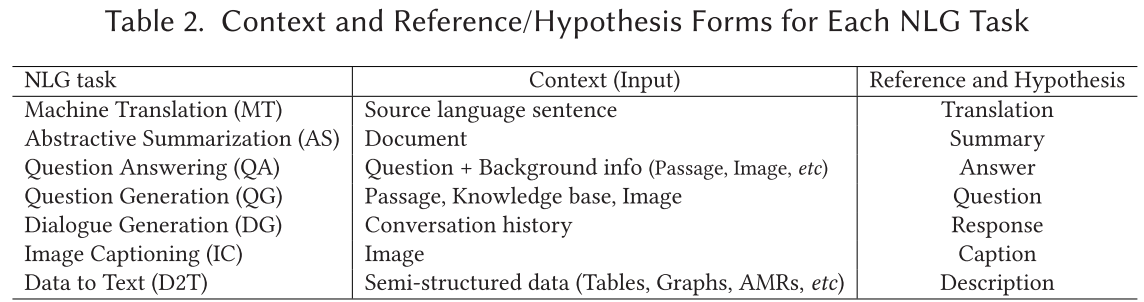
\includegraphics[width=\linewidth]{img/nlg1.png}

\begin{tikzpicture}[overlay, remember picture] 
\node at (current page.north east)[ref] {\fullcite{Sai.et.al.2023.CSUR} \par};
\end{tikzpicture}

\end{frame}


\begin{frame}{Evaluating text generation is hard}
	
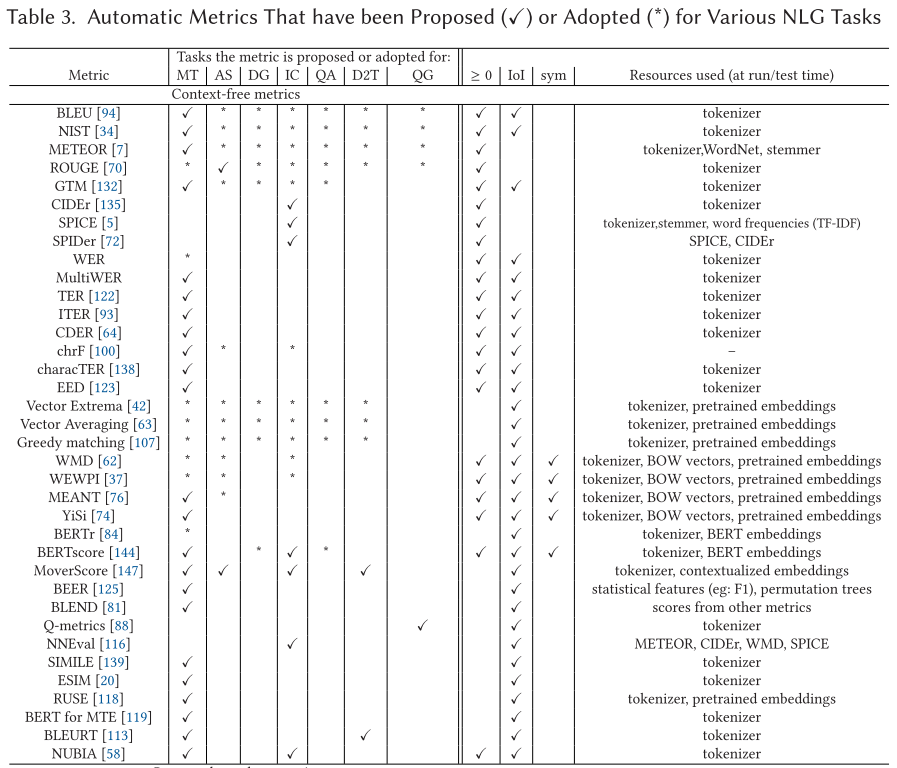
\includegraphics[trim={0 12.2cm 0 0},clip,width=1.2\linewidth]{img/nlg2.png}
	
\end{frame}


\begin{frame}{BLEU (Bilingual Evaluation Understudy)}

Almost first and most popular metric for MT

\begin{itemize}
	\item Precision-based metric that computes the n-gram overlap between the reference and the hypothesis
	\item In particular, BLEU is the ratio of the number of overlapping n-grams to the total number of n-grams in the hypothesis.
\end{itemize}


Corpus-level metric, i.e., BLEU gives a score over the entire corpus (as opposed to scoring individual sentences)

Major drawbacks of BLEU: (i) it does not take recall into account and (ii) it only allows exact n-gram matching

\begin{tikzpicture}[overlay, remember picture] 
\node at (current page.north east)[ref] {\fullcite{Papineni.et.al.2002.ACL} \par};
\end{tikzpicture}

\end{frame}


\begin{frame}{ROUGE (Recall-Oriented Understudy\\ for Gisting Evaluation)}
	
ROUGE metric includes a set of variants: ROUGE-N, ROUGE-L, ROUGE-W, and ROUGE-S

\begin{itemize}
	\item ROUGE-N is similar to BLEU-N in counting the n-gram matches between the hypothesis and reference, however, it is a recall-based measure unlike BLEU which is precision-based
	\item ROUGE-L measures the longest common subsequence (LCS) between a pair of sentences	
\end{itemize}

\begin{tikzpicture}[overlay, remember picture] 
	\node at (current page.north east)[ref] {\fullcite{Lin.2004} \par};
\end{tikzpicture}


\end{frame}


\subsection{Caveats of NLP benchmarking}


\begin{frame}{The `gold' data paradigm might not always fit}

The assumption of a ground truth makes sense when humans highly agree on the answer

\begin{itemize}
	\item ``Does this image contain a bird?"
	\item ``Is `learn' a verb?"
	\item ``What is the capital of Italy?"
\end{itemize}

This assumption often does not make sense, especially when language is involved

\begin{itemize}
	\item ``Is this comment toxic?"
\end{itemize}

\emph{Human label variation impacts all steps of the traditional ML pipeline, and is an opportunity, not a problem}

\begin{tikzpicture}[overlay, remember picture] 
	\node at (current page.north east)[ref] {\fullcite{Plank.2022.EMNLP} \par};
\end{tikzpicture}

\end{frame}

\begin{frame}{ Human annotators are biased}

Datasets are often constructed using a small number of annotators, and humans are biased

\begin{itemize}
	\item Concerns about data diversity, especially when workers freely generate sentences
	\item Models do not generalize well to examples from annotators that did not contribute to the training set
\end{itemize}

\begin{tikzpicture}[overlay, remember picture] 
	\node at (current page.north east)[ref] {\fullcite{Geva.et.al.2019.EMNLP} \par};
\end{tikzpicture}

\end{frame} \begin{frame}{Artifacts in datasets}

Datasets have artifacts (spurious statistics) that can be exploited

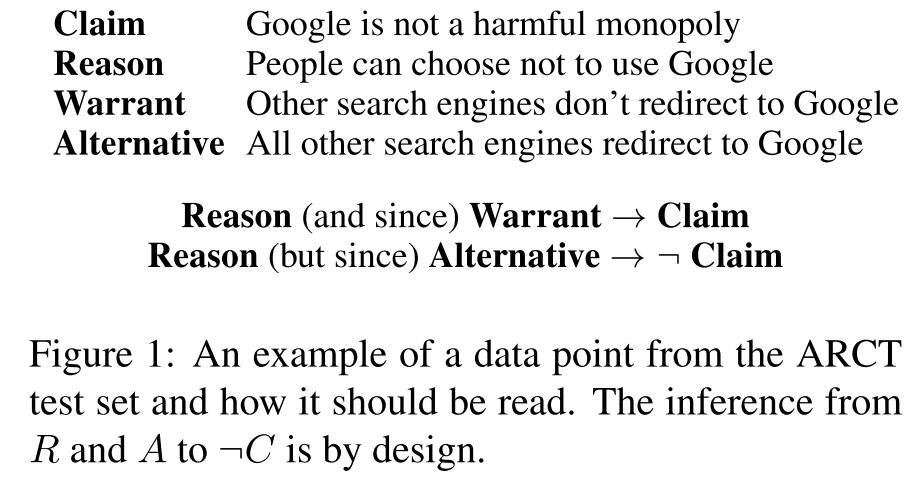
\includegraphics[width=8cm]{img/arct.png}



\begin{tikzpicture}[overlay, remember picture] 
	\node at (current page.north east)[ref] {\fullcite{Habernal.et.al.2018.NAACL.ARCT} 
		\bigskip \newline	
		\fullcite{Niven.Kao.2019.ACL} \par};
\end{tikzpicture}


\end{frame}


\begin{frame}{License and credits}
	
	\begin{columns}
		\begin{column}{0.7\textwidth}
			Licensed under Creative Commons Attribution-ShareAlike 4.0 International (CC BY-SA 4.0)
		\end{column}
		\begin{column}{0.2\textwidth}
			
\includegraphics[width=0.9\linewidth]{img/cc-by-sa-icon.pdf}
		\end{column}
	\end{columns}
	
	\bigskip
	
	Credits
	
	\begin{scriptsize}
		
		Ivan Habernal
		
		Content from ACL Anthology papers licensed under CC-BY \url{https://www.aclweb.org/anthology}
		
	\end{scriptsize}
	
\end{frame}


\end{document}

